\documentclass[12pt]{article}

\usepackage[T1]{fontenc} % used for font (special symbols like _)
% \usepackage{listings} % could be used instead of minted
% \usepackage{xcolor} % used to define custom colors and use already defined ones
\usepackage{hyperref} % used for links in table of contents
\usepackage{tocbibind} % used for depth in table of contents
\usepackage[a4paper, margin=3cm]{geometry} % increase page margins
\usepackage{minted} % used for code highlighting
\usepackage{blindtext} % used for inserting lorem ipsum (\blindtext)
\usepackage[most]{tcolorbox} % used for notes
\usepackage{graphicx} % used for inserting images
% \usepackage{float} % used for fixing image in place
\usepackage{enumitem} % used for removing spaces between lines

\author{
  Jakub Czermański\\
  \texttt{193105}
  \and
  Paweł Blicharz\\
  \texttt{193193}
}
\date{02.05.2024}
\title{Using CNNs to classify people in Famous48 dataset - Subject 12c}

% Define how code should be displayed
% https://www.overleaf.com/learn/latex/Code_Highlighting_with_minted
% for minted, removes heading spaces: https://tex.stackexchange.com/questions/423275/minted-aligning-code-fragments-left

% remove spaces between items in lists:
\setlist{noitemsep}

\setcounter{tocdepth}{3} % set depth in the table of contents to 3
\hypersetup{
  colorlinks=true,
  allcolors=black,
  % linkcolor=blue,
  % filecolor=magenta,
  % urlcolor=cyan,
  % pdftitle={An Example},
  % pdfpagemode=FullScreen,
}

\makeatletter
\NewDocumentCommand{\mynote}{+O{}+m}{%
  \begingroup
  \tcbset{%
    noteshift/.store in=\mynote@shift,
    noteshift=1.5cm
  }
  \begin{tcolorbox}[nobeforeafter,
    enhanced,
    sharp corners,
    toprule=1pt,
    bottomrule=1pt,
    leftrule=0pt,
    rightrule=0pt,
    colback=yellow!20,
    #1,
    left skip=\mynote@shift,
    right skip=\mynote@shift,
    overlay={\node[right] (mynotenode) at ([xshift=-\mynote@shift]frame.west) {\textbf{Note:}} ;},
    ]
    #2
  \end{tcolorbox}
  \endgroup
  }
\makeatother


\begin{document}
  \pagenumbering{gobble}
  \maketitle
  \newpage
  \tableofcontents
  \newpage
  \pagenumbering{arabic}

  \section{Introduction}
    Lorem ipsum
    \subsection*{Data description}
      famous48 is a set of example images contained faces of 48 famous persons like sportsmens, politicians, actors or television stars. It was divided into 3 files: x24x24.txt, y24x24.txt, z24x24.txt, each containing 16 personal classes.
      \\\\
      Attributes description:
      \begin{itemize}
        \item a1 - face containing flag: (1-with face, 0-without face)
        \item a2 - image number in current class (person) beginning from 0
        \item a3 - class (person) number beginning from 0
        \item a4 - sex (0 - woman, 1 - man)
        \item a5 - race (0- white, 1 - negro, 2 - indian, ...)
        \item a6 - age (0 - baby, 1 - young, 2 - middle-age, 3 - old)
        \item a7 - binokulars (0 - without, 1 - transparent, 2 - dark)
        \item a8 - emotional expression (not state!) (0 - sad, 1 - neutral, 2 - happy)
      \end{itemize}
    % asdf
    % \\\\
    \mynote{Full code can be found in \textit{notebook\_keras.ipynb}. Due to limited space, we provide here only the most important code.}
  \section{Libraries used}
    Firstly, we import all our libraries:
    \inputminted[linenos]{python}{code/imports.py}
  \section{File loading}
    This is our code for loading files and we will not change it throughout our journey:
    \inputminted[linenos]{python}{code/loading.py}
  \section{Testing}
    Here are our all attempts at finding the best model. We tried out different architectures and hyperparameters to achieve that goal.
    \subsection{Architectures}
      \subsubsection{AlexNet}
        Firstly, we implemented AlexNet model (\url{https://papers.nips.cc/paper_files/paper/2012/hash/c399862d3b9d6b76c8436e924a68c45b-Abstract.html})
        which won the 2012 ILFRC challenge. Here is our model in python code, after downscaling it and changing some parameters:
        \inputminted[linenos]{python}{code/alexnet.py}
        \paragraph{Hyperparameters \& methods used:}
          \begin{itemize}
            \item \textit{optimizer}: Adam, with \textit{learning rate} = 0.001
            \item \textit{epochs} = 250
            \item \textit{batch size} = 200
            \item \textit{validation set size} = 20\% of the training set
            \item \textit{shuffle} the training data before each epoch
            \item L2 regularization for convolutional layers: $l = 0.0006$
            \item L2 regularization for the dense layer: $l = 0.01$
          \end{itemize}
        \paragraph{Results:} (rounded to 3 decimal places)
          \begin{itemize}
            \item train set accuracy: 0.896
            \item train loss: 0.775
            \item validation set accuracy: 0.81
            \item validation set loss: 1.115
            \item test set accuracy: \textbf{0.8}
            \item test set loss: 1.137
          \end{itemize}
              \begin{figure}[H]
                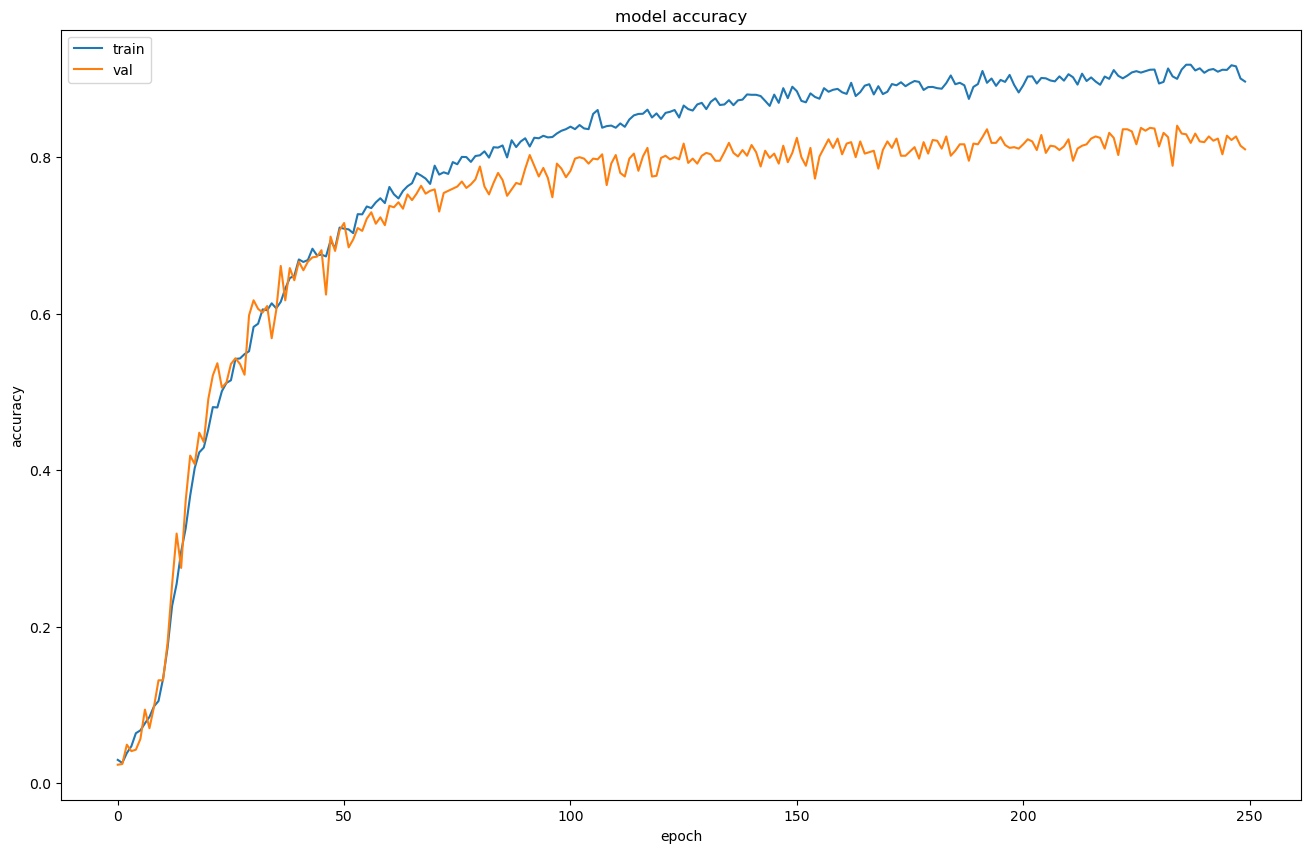
\includegraphics[width=\linewidth]{images/alex-net.png}
                \caption{Model accuracy for AlexNet architecture - training \& validation sets}
                \label{fig:alex-net}
              \end{figure}
        \paragraph{Conclusions:} \mbox{} \\\\
        We decided that 80\% is not enough so we did not tune hyperparameters.
      \subsubsection{LeNet-5}
        Next, we decided to used LeNet-5 architecture, presented below:
        \inputminted[linenos]{python}{code/lenet.py}
        \paragraph{Hyperparameters \& methods used:}
        \begin{itemize}
          \item \textit{optimizer}: Adam, with \textit{learning rate} = 0.001
          \item \textit{epochs} = 100
          \item \textit{batch size} = 200
          \item \textit{validation set size} = 20\% of the training set
          \item \textit{shuffle} the training data before each epoch
          \item L2 regularization for convolutional layers: $l \approx 0.00091$
          \item L2 regularization for the dense layer: $l \approx ?(to-do)$
        \end{itemize}
        \paragraph{Results:} (rounded to 2(to-do: change to 3) decimal places)
          \begin{itemize}
            \item train set accuracy: 0.92
            \item train loss: ?
            \item validation set accuracy: 0.82
            \item validation set loss: ?
            \item test set accuracy: \textbf{0.82}
            \item test set loss: ?
          \end{itemize}
              \begin{figure}[H]
                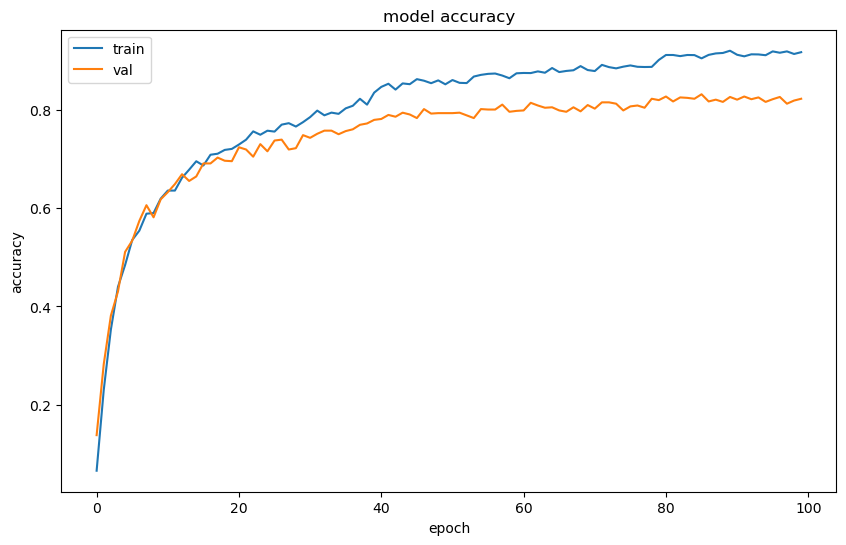
\includegraphics[width=\linewidth]{images/lenet.png}
                \caption{Model accuracy for LeNet-5 architecture - training \& validation sets}
                \label{fig:lenet}
              \end{figure}
        \paragraph{Conclusions:} \mbox{} \\\\
        The model after 20 epochs starts overfitting and validation set's accuracy improves very slowly.
    \section{Final model}


\end{document}
